\documentclass[letterpaper,11pt]{article}

% --- PAQUETES DE IDIOMA
\usepackage[spanish,mexico]{babel}
\usepackage[utf8]{inputenc}
\usepackage{csquotes}
\usepackage{iftex}

\PassOptionsToPackage{table}{xcolor}
\usepackage{pdfpages}

% --- PAQUETES MATEMÁTICOS --
\usepackage{amsmath}
\usepackage{cancel}
\usepackage{mathrsfs}

% --- PAQUETES GRÁFICOS Y DE DISEÑO ---
\usepackage{graphicx}
\usepackage{float}
\usepackage{placeins}
\usepackage{subcaption}
\usepackage[table]{xcolor}
\usepackage{makecell}
\usepackage{array}
\usepackage{tikz}
\usetikzlibrary{shapes.geometric, shapes.multipart, positioning, arrows.meta, calc, shadows, decorations.pathreplacing,babel}

% --- LISTAS ---
\usepackage{enumitem}

% --- PAQUETES DE CÓDIGO ---
\usepackage{listings}
% Configuración del estilo de listings
\definecolor{codebg}{rgb}{0.95,0.95,0.95}   
\definecolor{keyword}{rgb}{0.0,0.2,0.6}     
\definecolor{comment}{rgb}{0.25,0.5,0.35}   
\definecolor{string}{rgb}{0.6,0.0,0.0}      
\definecolor{number}{rgb}{0.5,0.0,0.5}      
\definecolor{codegray}{rgb}{0.5,0.5,0.5}
\definecolor{codepurple}{rgb}{0.58,0,0.82}
\definecolor{backcolour}{rgb}{0.95,0.95,0.95}

\lstset{
  backgroundcolor=\color{backcolour},
  basicstyle=\ttfamily\small,
  keywordstyle=\color{blue}\bfseries,
  stringstyle=\color{codepurple},
  commentstyle=\color{codegray}\itshape,
  numbers=left,
  numberstyle=\tiny\color{codegray},
  frame=single,
  rulecolor=\color{black},
  breaklines=true,
  tabsize=4,
  showstringspaces=false,
  literate={á}{{\'a}}1
           {é}{{\'e}}1
           {í}{{\'i}}1
           {ó}{{\'o}}1
           {ú}{{\'u}}1
           {Á}{{\'A}}1
           {É}{{\'E}}1
           {Í}{{\'I}}1
           {Ó}{{\'O}}1
           {Ú}{{\'U}}1
           {ñ}{{\~n}}1
           {Ñ}{{\~N}}1
           {¿}{{\textquestiondown}}1
           {¡}{{\textexclamdown}}1
}

% Estilo para código en C
\lstdefinestyle{cstyle}{
  language=C,
  backgroundcolor=\color{backcolour},
  basicstyle=\ttfamily\small,
  keywordstyle=\color{blue}\bfseries,
    keywordstyle=[2]\color{yellow!70!orange}\bfseries,
    morekeywords=[2]{MPI_Init,MPI_Comm_size,MPI_Comm_rank,MPI_Send,MPI_Recv,MPI_Scatter,MPI_Gather,MPI_Bcast,MPI_Reduce,MPI_Finalize},
    emph={printf},
    emphstyle=\color{blue}\bfseries,
  stringstyle=\color{codepurple},
  commentstyle=\color{codegray}\itshape,
  numbers=left,
  numberstyle=\tiny\color{codegray},
  frame=single,
  rulecolor=\color{black},
  breaklines=true,
  tabsize=4,
  showstringspaces=false
}

% Definición del lenguaje Python para listings
\lstdefinelanguage[LAB]{Python}{
    morekeywords={False, None, True, and, as, assert, async, await, break,
                                class, continue, def, del, elif, else, except, finally,
                                for, from, global, if, import, in, is, lambda, nonlocal,
                                not, or, pass, raise, return, try, while, with, yield,
                                machine, Pin, PWM, ADC, Timer, sleep_ms, sleep_us},
    morecomment=[l]{\#},
    morestring=[b]",
    morestring=[b]',
    sensitive=true
}

% Estilo para salidas de consola/terminal
\lstdefinestyle{output}{
  backgroundcolor=\color{black!5},
  basicstyle=\ttfamily\footnotesize,
  numbers=none,
  frame=single,
  rulecolor=\color{black!30},
  breaklines=true,
  tabsize=4,
  showstringspaces=false,
  xleftmargin=0.5cm,
  xrightmargin=0.5cm
}

% --- ESTILOS PARA DIAGRAMAS DE FLUJO (TIKZ) ---
\tikzset{
  startstop/.style={rectangle, rounded corners, minimum width=3cm, minimum height=1cm,text centered, draw=black, fill=red!30},
  process/.style={rectangle, minimum width=3cm, minimum height=1cm, text centered, draw=black, fill=orange!30},
  decision/.style={diamond, aspect=2, minimum width=3cm, minimum height=1cm, text centered, draw=black, fill=green!30},
  io/.style={trapezium, trapezium left angle=70, trapezium right angle=110, minimum width=3cm, minimum height=1cm, text centered, draw=black, fill=blue!30},
  arrow/.style={thick,->,>=stealth}
}


\definecolor{azulresultado}{HTML}{0072C6}
\definecolor{rojoacarreo}{HTML}{FF0000}

% --- RUTAS DE IMÁGENES ---
\graphicspath{{img/}{portada_img/}}

\definecolor{armblue}{RGB}{0, 113, 188}

% --- ÍNDICE CON PUNTOS ---
\usepackage{tocloft}
\renewcommand{\cftsecleader}{\cftdotfill{\cftdotsep}}

% --- CONFIGURACIÓN DE PÁGINA (GEOMETRÍA) ---
\usepackage[
    left=25mm, 
    right=25mm,
    top=35mm,
    bottom=30mm,
    headheight=77pt, 
    papersize={21.59cm,27.94cm}
]{geometry}

% --- FORMATO DE TEXTO ---
\usepackage{setspace}
\onehalfspacing
\usepackage{parskip} 
\usepackage{microtype}  

% --- VARIABLES GLOBALES ---
\newcommand{\materia}{}

% --- ENCABEZADOS Y PIES DE PÁGINA ---
\usepackage{fancyhdr}
\pagestyle{fancy}
\fancyhf{} 
\fancyhead[L]{
\includegraphics[height=1.5cm]{portada_img/der.png}}
\fancyhead[R]{
\includegraphics[height=1.5cm]{portada_img/izq.png}}
\fancyfoot[C]{\thepage} 
\renewcommand{\headrulewidth}{0.4pt} 
\renewcommand{\footrulewidth}{0pt}  

% --- BIBLIOGRAFÍA ---
%\usepackage[backend=biber, style=apa, sortcites, url=true]{biblatex}
%\addbibresource{referencias.bib}

% --- HIPERVÍNCULOS ---
\usepackage{hyperref}
\usepackage{xurl}
\hypersetup{
    colorlinks=true,
    linkcolor=blue,
    citecolor=blue,
    filecolor=magenta,
    urlcolor=cyan
}


% Las capturas conservan sus nombres originales y su proporción.
\newcommand{\captura}[4][\textwidth]{%
\begin{figure}[H]
\centering
\includegraphics[width=#1,height=0.78\textheight,keepaspectratio]{\detokenize{image/#2}}
\caption{#3}\label{#4}
\end{figure}}
\begin{document}
\thispagestyle{empty} % Sin encabezado ni pie en la portada

% --- ENCABEZADO DE PORTADA (TABLA DE 3 COLUMNAS) ---
\begin{center}
    % La tabla usa 'm' para centrar verticalmente las imágenes y el texto
    \begin{tabular}{m{0.15\textwidth} m{0.60\textwidth} m{0.15\textwidth}}
        % Logo Izquierdo (UNAM)
        
\includegraphics[width=2cm]{portada_img/der.png} & 
        
        % Título Central
        \centering\Huge\textbf{Universidad Nacional Autónoma de México} &
        
        % Logo Derecho (Facultad)
        \raggedleft
\includegraphics[width=2cm]{portada_img/izq.png}
    \end{tabular}
\end{center}

\vspace{0.3cm}

% --- INFORMACIÓN DEL REPORTE ---
\begin{center}
    {\LARGE \textbf{Facultad de Ingeniería}}\\[1cm]

    {\LARGE \textbf{Alumno:}}\\[0.3cm]
    {\Large Lara Hernandez Angel Husiel - 320060829} \\[1cm]


    {\LARGE \textbf{Arquitectura Cliente-Servidor}} \\[1cm]

	{\LARGE Grupo: 02 - Semestre: 2027-1} \\[1cm]
    
    {\LARGE \textbf{Tarea 4:}}\\[0.5cm]

    {\LARGE {Sockets Internet y cola de espera.}}\\[1cm]

    {\LARGE \textbf{Profesor:}}\\[0.2cm]
    {\Large MTRO. CARLOS ALBERTO ROMAN ZAMITIZ}\\[1cm]

    {\Large \textbf{Fecha de realización:}}\\[0.2cm]
    {\Large 8 de octubre del 2026}
\end{center}
\newpage
{\hypersetup{linkcolor=black}\tableofcontents}
\thispagestyle{empty}
\newpage
\setcounter{page}{1}
\singlespacing

\section{Investigacion sobre los comandos y la funcion sk\_acceptq\_is\_full()}

\subsection{Funcionamiento del programa:}

\subsection{Función sk\_acceptq\_is\_full():}

Primero que nada, en este caso el codigo de esta funcion, esta en :
\texttt{include/net/sock.h}, esta es una función interna del 
núcleo que consulta la cola Accept del socket.

Para la parte de \texttt{sk\_ack\_backlog} lleva la 
cantidad de conexiones pendientes y 
\texttt{sk\_max\_ack\_backlog} contiene el límite de la cola. 
La comprobación se realiza de la siguiente forma:

\begin{lstlisting}[style=cstyle,caption={Comparación utilizada para revisar la cola Accept.}]
static inline bool sk_acceptq_is_full(const struct sock *sk)
{
    return READ_ONCE(sk->sk_ack_backlog) >
           READ_ONCE(sk->sk_max_ack_backlog);
}
\end{lstlisting}

Ahora bien, en el cso de la funcion utiliza \texttt{>}, esto basado en 
backlog 1, la comparación $1 > 1$ es falsa y 
puede entrar otra conexión pendiente; 
con dos, $2 > 1$ es verdadera. 

Por lo tanto, en esta prueba el primer cliente es atendido y 
los siguientes dos esperan, pero 
ya para el cuarto se ve el desbordamiento. 

\subsection{Investigacion de cat /proc/sys/net/ipv4/tcp\_syncookies:}

\begin{lstlisting}[style=output]
cat /proc/sys/net/ipv4/tcp_syncookies
\end{lstlisting}
Para el caso de este comando, \texttt{cat} muestra el valor actual de un 
parámetro TCP expuesto por Linux en \texttt{/proc/sys/net/ipv4/}. 
La consulta no cambia la configuración. En mi linux se obtuvo 1 
antes de realizar los ajustes.

Ahora bien, \texttt{tcp\_syncookies} controla las SYN cookies, 
que sirven como protección cuando se desborda la cola SYN. 
El valor 0 las desactiva, 1 permite utilizarlas ante ese desbordamiento 
y 2 las genera de forma incondicional.

\subsection{Investifacion  cat /proc/sys/net/ipv4/tcp\_syn\_retries:}

\begin{lstlisting}[style=output]
cat /proc/sys/net/ipv4/tcp_syn_retries
\end{lstlisting}

Por otra parte, este comando consulta el límite de retransmisiones 
del SYN durante un intento de conexión activa, en el caso de mi linux
se obtuvo 6, esto es con relacion a los intentos que hace el 
cliente cuando la conexión no se completa; no significa que el 
servidor admita seis clientes.

Lo que hace el 1 es que reduce ese límite. 
Este parámetro es distinto de \texttt{tcp\_synack\_retries}, 
que corresponde a las retransmisiones SYN+ACK del servidor. 
El cambio tampoco modifica el backlog.

\section{Codigo e implementacion:}


Al iniciar se crea el socket por medio de \texttt{socket()}, después se coloca la dirección y el puerto en la estructura \texttt{sockaddr\_in}. La llamada \texttt{bind()} asocia el socket con las direcciones locales del servidor, esto debido a que se utiliza \texttt{INADDR\_ANY}. Por último se llama a \texttt{listen()} y el proceso espera una conexión en \texttt{accept()}.

Cuando el primer cliente es aceptado, el programa entra a un segundo ciclo que utiliza \texttt{recv()}. Lo que sucede aquí es que el servidor permanece ocupado con ese cliente mientras no se desconecte. Si no se envían datos, \texttt{recv()} queda bloqueada, por lo que el proceso no regresa a ejecutar \texttt{accept()} para los siguientes clientes. No obstante, el sistema operativo continúa procesando las solicitudes de conexión y administra las colas TCP.

La cola SYN contiene solicitudes cuyo establecimiento todavía no se ha completado desde el lado del servidor. En una conexión normal, el cliente envía SYN, el servidor contesta SYN+ACK y el cliente responde ACK. Cuando el servidor procesa este último paso, la conexión puede pasar a la cola Accept.

La cola Accept contiene conexiones establecidas que todavía no han sido retiradas por el programa mediante \texttt{accept()}. Esto es importante, porque el mensaje de conexión exitosa de \texttt{nc} corresponde al establecimiento TCP visto por el cliente, y por sí solo no demuestra que el servidor ya esté atendiendo a ese cliente.


\subsection{Configuracion de l terminal:}

En este caso, \texttt{sudo} permite ejecutar el cambio con 
permisos de administrador, mientras que \texttt{sysctl -w} 
escribe el valor del parámetro del sistema en ejecución. 
El primer comando desactiva las SYN cookies y el segundo reduce 
los reintentos SYN. Los cambios se realizan para observar el 
comportamiento del laboratorio y al terminar se deben regresar 
a los valores guardados, sin modificar los archivos de configuración 
permanente.

\begin{lstlisting}[style=output]
sudo sysctl -w net.ipv4.tcp_syncookies=0
sudo sysctl -w net.ipv4.tcp_syn_retries=1
\end{lstlisting}

Ahora bien, el compilador regresó a la línea de comandos sin mostrar errores. Después se consultó cada parámetro por separado, donde se obtuvieron los valores originales 1 y 6:
\begin{lstlisting}[style=output]
cat /proc/sys/net/ipv4/tcp_syncookies
1
cat /proc/sys/net/ipv4/tcp_syn_retries
6
\end{lstlisting}

\begin{figure}[H]
  \centering
  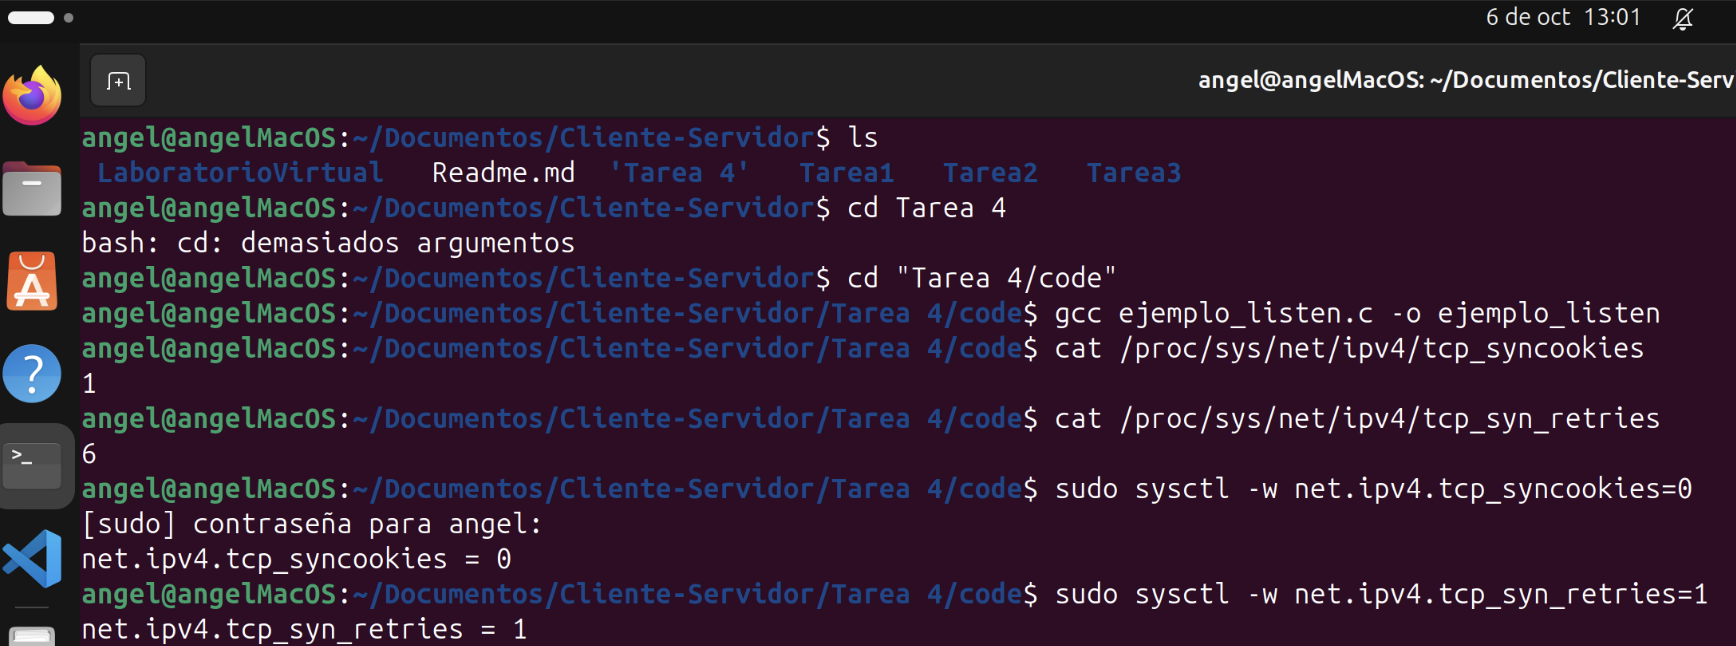
\includegraphics[width=0.7\textwidth]{image/image2.png}
  \caption{Compilación, consulta de parámetros, aplicación de los ajustes y restauración de los valores originales.}
\end{figure}

Con los comandos sudo, puesto correspondientemente, ahora el \texttt{tcp\_syncookies} tiene un valor 
de 0 y \texttt{tcp\_syn\_retries} de 1. Esto permite observar el comportamiento del servidor cuando se desborda la cola SYN, 
además de reducir el tiempo de espera del cuarto cliente.


\subsection{Compilación del servidor:}
Desde la raíz del repositorio se ejecutan los siguientes comandos dentro de Linux:
\begin{lstlisting}[style=output]
cd "Tarea 4/code"
gcc ejemplo_listen.c -o ejemplo_listen
./ejemplo_listen 4898
\end{lstlisting}

\begin{figure}[H]
  \centering
  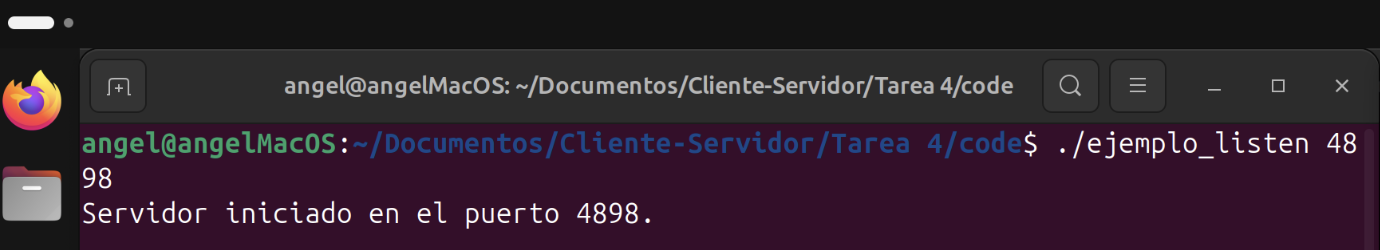
\includegraphics[width=0.7\textwidth]{image/image1.png}
  \caption{Compilación y ejecución del servidor en el puerto 4898.}
\end{figure}

\subsection{Servidor y primera conexión:}

En la terminal de la izquierda se ejecutó \texttt{./ejemplo\_listen 4898}, 
donde el programa mostró que había iniciado en el puerto 4898 y 
que estaba esperando en \texttt{accept()}. 
Por otra parte, en la terminal de la derecha se ejecutó 
\texttt{nc -v 127.0.0.1 4898}, que mostró el mensaje de conexión exitosa.

\captura{Captura de pantalla 2026-10-06 a la(s) 1.02.09 p.m..png}{Servidor en el puerto 4898 y primer cliente conectado.}{fig:primera-conexion}

Lo que vemos aquí es que el servidor imprime el cliente fue aceptado

y señaló que estaba ocupado atendiendo a ese cliente. 
Esto permite comprobar que la primera conexión sí fue 
retirada de la cola por medio de \texttt{accept()}. 
Como el cliente permaneció abierto sin enviar datos, 
el servidor continuó esperando en \texttt{recv()}.



\subsection{Ejecución de los cuatro clientes:}
Para los clientes se abren cuatro terminales, ejecutando el siguiente comando en cada una, de forma consecutiva:
\begin{lstlisting}[style=output]
nc -v 127.0.0.1 4898
\end{lstlisting}
El parámetro \texttt{-v} muestra información del intento de conexión. 
El primer cliente debe mantenerse abierto para que el servidor 
permanezca ocupado. Después se ejecutan los clientes segundo, 
tercero y cuarto, manteniendo las terminales visibles para 
comparar los resultados.

Ahora bien, se ve el servidor en la parte superior izquierda y el 
primer cliente en la parte superior derecha. 
Los clientes segundo y tercero se encuentran en las terminales inferiores, 
donde ambos mostraron que la conexión TCP fue exitosa. 
No obstante, el servidor solamente mostró una conexión 
aceptada, por lo que esos dos clientes todavía estaban 
esperando su turno de atención.

\captura{Captura de pantalla 2026-10-06 a la(s) 1.04.21 p.m..png}{Servidor y cuatro clientes: tres conexiones exitosas y un intento que terminó por tiempo de espera.}{fig:cuatro-clientes}


Por otra parte, la terminal pequeña de la derecha corresponde 
al cuarto cliente. En este caso, el comando terminó 
con \texttt{Connection timed out}, lo que significa que no pudo 
completar la conexión dentro del tiempo de espera. No se observó un 
rechazo inmediato; el resultado que se obtuvo fue el agotamiento del 
tiempo de conexión.


\subsection{Consulta de las conexiones con ss:}
En una sexta terminal se ejecuta:
\begin{lstlisting}[style=output]
ss -atnp | grep :4898
watch -n 1 "ss -atn 'sport = :4898'"
\end{lstlisting}

\begin{figure}[H]
  \centering
    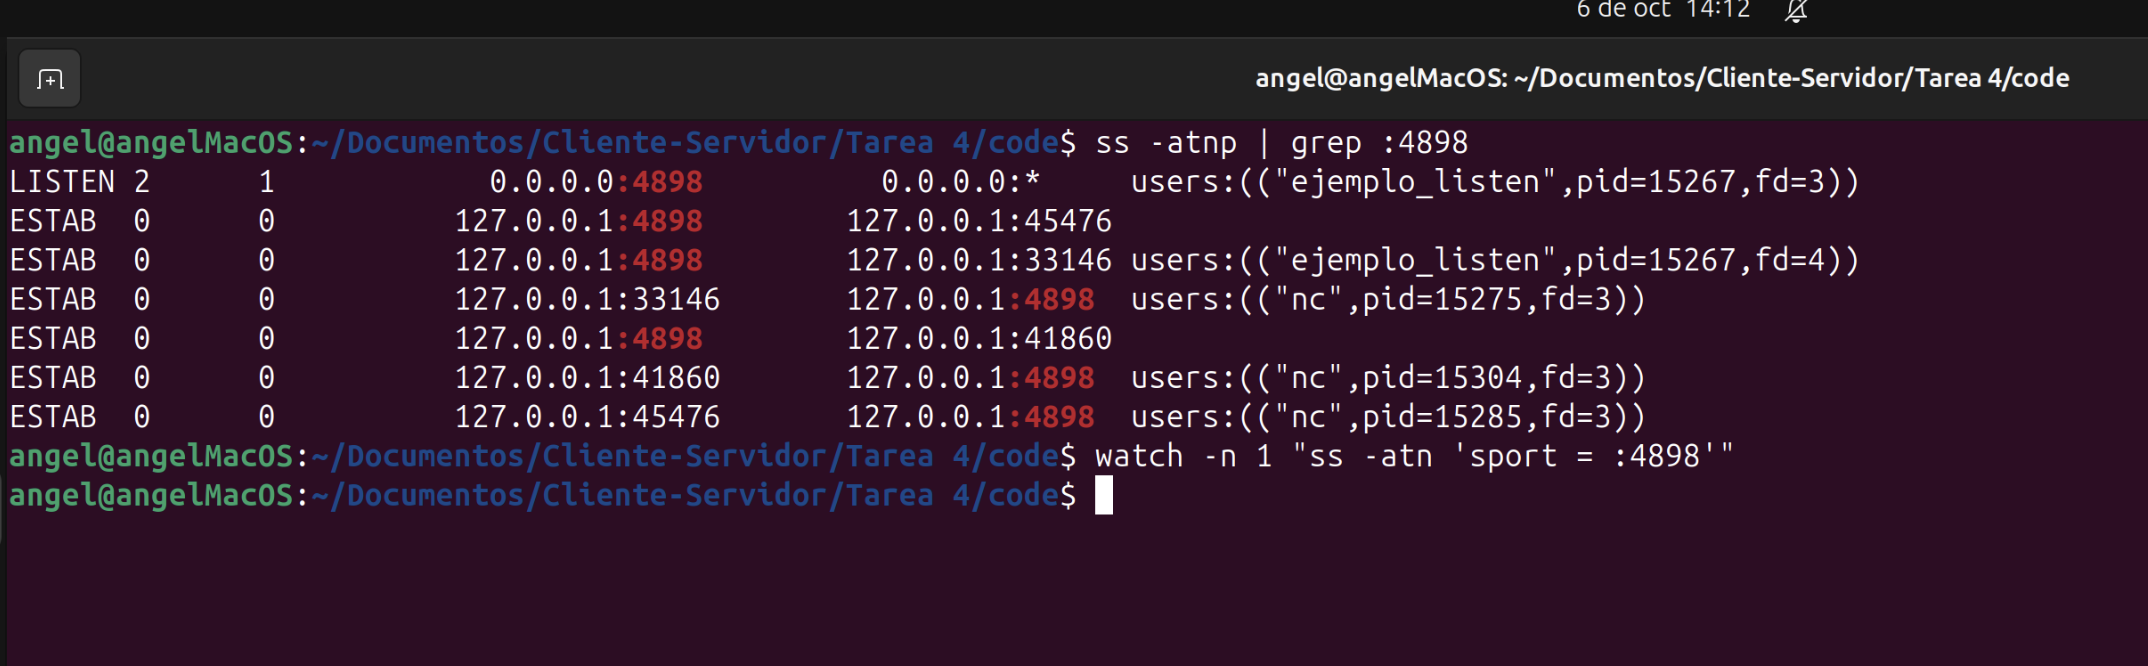
\includegraphics[width=0.7\textwidth]{image/image3.png}
  \caption{Vista de la finalizacion del comando, una vez cerrado els ervidor.}
\end{figure}

El primer comando muestra los sockets TCP relacionados con el puerto, junto con la información de proceso que esté disponible para el usuario. El segundo actualiza cada segundo los sockets cuyo puerto local es 4898, esto para ver el estado del servidor.

En la fila \texttt{LISTEN}, la columna \texttt{Recv-Q} indica cuántas conexiones están esperando a \texttt{accept()}, mientras que \texttt{Send-Q} muestra el backlog configurado. Por lo tanto, una fila \texttt{LISTEN 2 1} permite observar dos conexiones pendientes con backlog 1. En las filas \texttt{ESTAB}, esas mismas columnas representan bytes, por lo que no se interpretan como número de clientes.

\captura[0.70\textwidth]{Captura de pantalla 2026-10-06 a la(s) 1.02.40 p.m..png}{Monitor del puerto 4898: dos conexiones pendientes con backlog 1.}{fig:monitor}


Para el caso de esta consulta, lo que vemos en la fila 
\texttt{LISTEN} es un valor de 2 en \texttt{Recv-Q} y de 
1 en \texttt{Send-Q}. Esto indica que había dos conexiones 
esperando a que el programa volviera a ejecutar \texttt{accept()}, 
aunque el backlog del código tiene valor 1.

Además de eso, aparecen tres filas \texttt{ESTAB} del 
lado del servidor, relacionadas con los puertos de cliente 45476, 
33146 y 41860. La conexión que ya había sido aceptada correspondió al 
puerto 33146, mientras que las otras dos permanecieron en la cola.
En estas filas, los valores 0 de \texttt{Recv-Q} y \texttt{Send-Q} 
representan bytes; no significan que la cola Accept estuviera vacía.

\newpage
\textbf{Vista final:}

\begin{figure}[H]
  \centering
  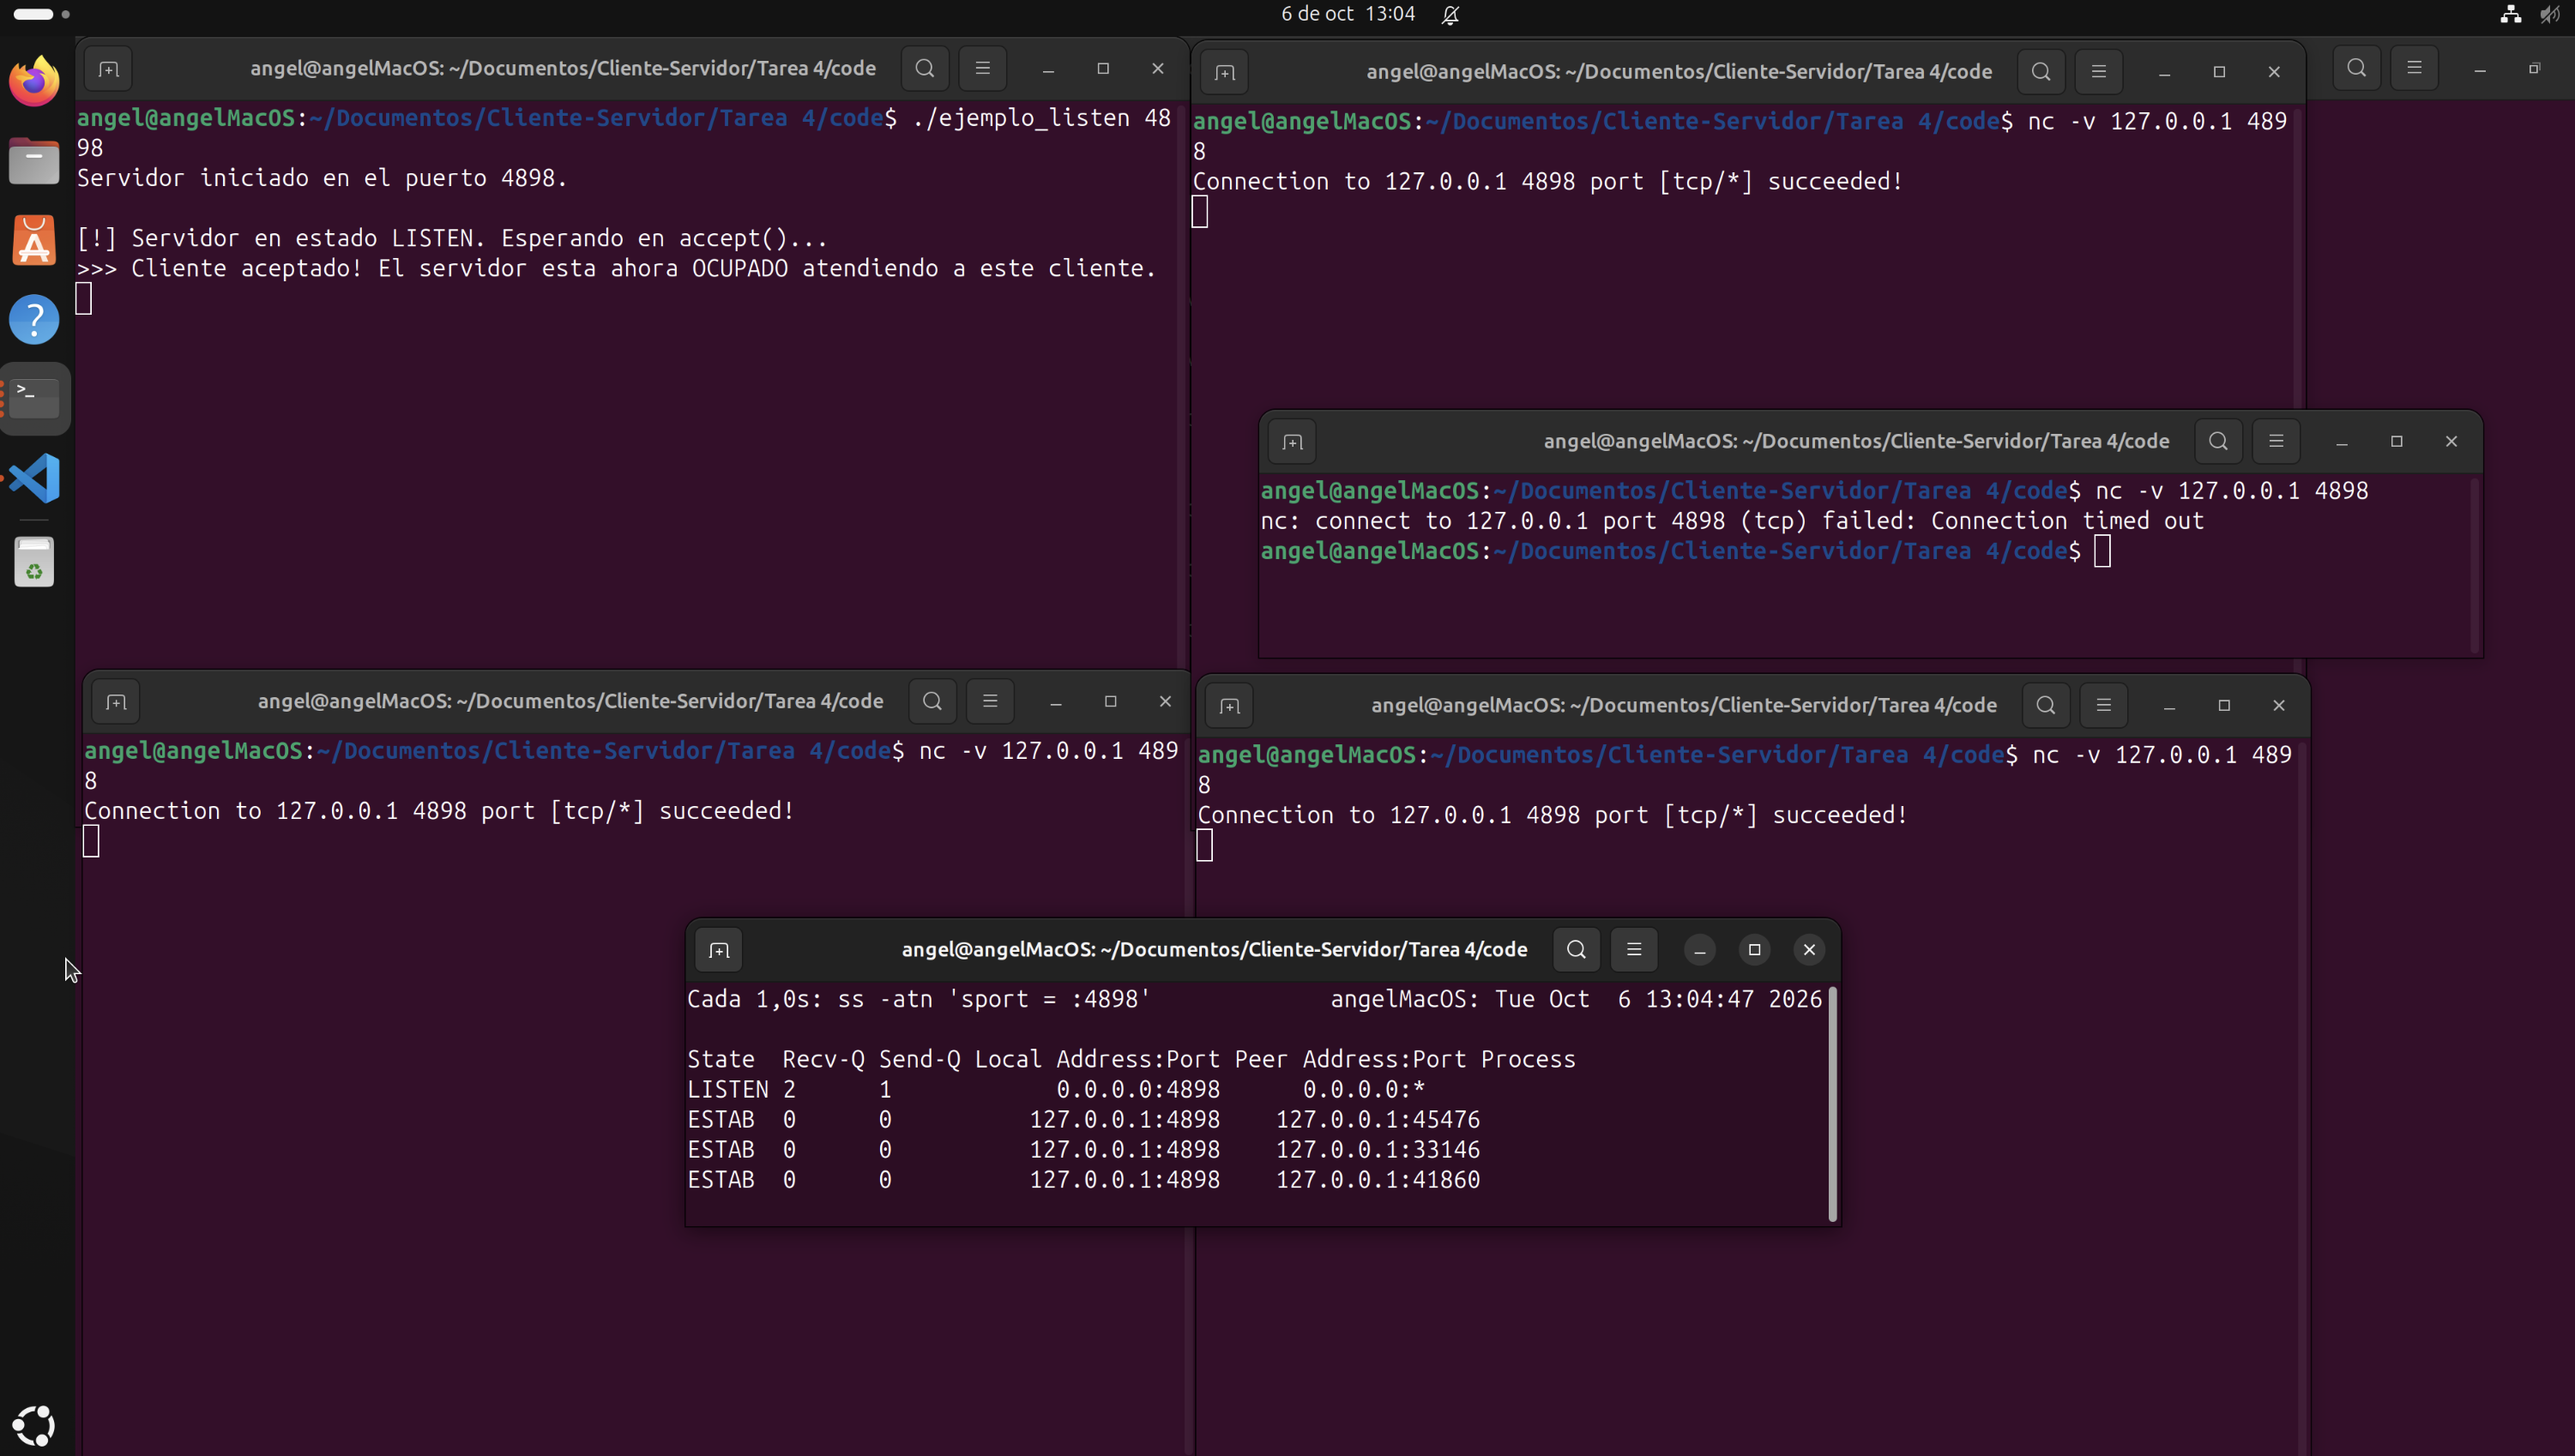
\includegraphics[width=0.8\textwidth]{image/image4.png}
  \caption{Vista conjunta del servidor, los cuatro clientes y el monitor de conexiones.}
\end{figure}


\subsection{Restauración de los parámetros:}
Al terminar los intentos de conexión se regresaron los valores originales, escribiendo cada comando por separado:
\begin{lstlisting}[style=output]
sudo sysctl -w net.ipv4.tcp_syncookies=1
sudo sysctl -w net.ipv4.tcp_syn_retries=6
cat /proc/sys/net/ipv4/tcp_syncookies
1
cat /proc/sys/net/ipv4/tcp_syn_retries
6
\end{lstlisting}

Como se ve en la parte final de la figura, 
la consulta devolvió 1 y 6. Por lo tanto, los cambios temporales 
quedaron restaurados y no se modificó la configuración permanente de la 
máquina virtual.

\begin{figure}[H]
  \centering
  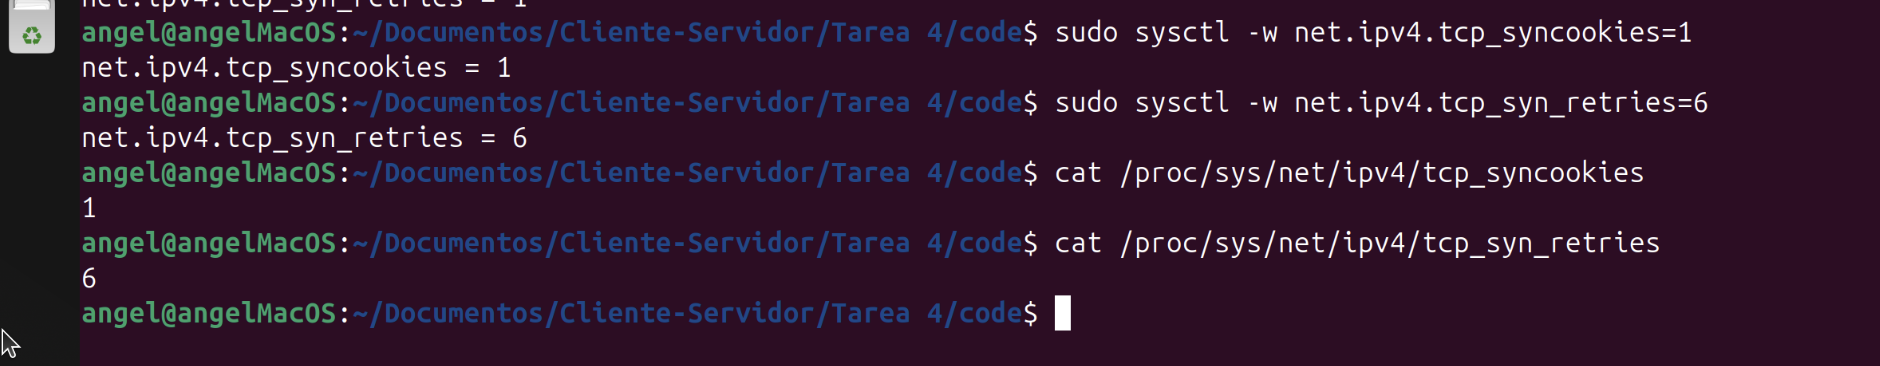
\includegraphics[width=0.7\textwidth]{image/image6.png}
  \caption{Restauracion de los parametros normales.}
\end{figure}

\section{Conclusión}
Para el caso de esta actividad se comprobó que el servidor atiende un cliente a la vez debido al ciclo con \texttt{recv()}, mientras que Linux mantiene otras conexiones esperando en la cola Accept. Aunque se configuró backlog 1, la consulta mostró dos conexiones pendientes, lo que coincide con la comparación estricta de \texttt{sk\_acceptq\_is\_full()}.

Ahora bien, los tres primeros clientes establecieron la conexión TCP, pero únicamente el primero fue atendido por el programa. El cuarto terminó con \texttt{Connection timed out}. Esto permite distinguir entre conectarse, quedar en espera y ser aceptado por la aplicación, además de explicar por qué fueron necesarios cuatro clientes para observar el desbordamiento en la máquina virtual utilizada.

\section{Referencias}
\begin{enumerate}
\item Linux Kernel. Documentación de parámetros IP sysctl: \texttt{tcp\_syncookies}, \texttt{tcp\_syn\_retries} y \texttt{tcp\_abort\_on\_overflow}.\\
\url{https://docs.kernel.org/networking/ip-sysctl.html}
\item OpenAnolis. TCP SYN Queue and Accept Queue Overflow Explained (2022).\\
\url{https://www.alibabacloud.com/blog/tcp-syn-queue-and-accept-queue-overflow-explained_599203}
\item Linux man-pages. Manual de TCP, interfaces de \texttt{/proc} y parámetros de conexión.\\
\url{https://man7.org/linux/man-pages/man7/tcp.7.html}
\end{enumerate}
\end{document}
